\PassOptionsToPackage{svgnames}{xcolor}
\documentclass[11pt]{article}
\usepackage[utf8]{inputenc}	% Para caracteres en español
\usepackage{amsmath,amsthm,amsfonts,amssymb,amscd}
\usepackage{multirow,booktabs}
\usepackage[table]{xcolor}
\usepackage{fullpage}
\usepackage{lastpage}
\usepackage{enumitem}
\usepackage{fancyhdr}
\usepackage{mathrsfs}
\usepackage{wrapfig}
\usepackage{setspace}
\usepackage{calc}
\usepackage{multicol}
\usepackage{cancel}
\usepackage[retainorgcmds]{IEEEtrantools}
\usepackage[margin=3cm]{geometry}
\usepackage{amsmath}
\newlength{\tabcont}
\setlength{\parindent}{0.0in}
\setlength{\parskip}{0.05in}
\usepackage{empheq}
\usepackage{framed}
\usepackage{tcolorbox}
\usepackage{xcolor}
\colorlet{shadecolor}{orange!15}
\tcbuselibrary{skins,breakable}
\usetikzlibrary{shadings,shadows}
\parindent 0in
\parskip 12pt
\geometry{margin=1in, headsep=0.25in}
\theoremstyle{definition}
\newtheorem{defn}{Definition}
\newtheorem{reg}{Rule}
\newtheorem{exer}{Exercise}
\newtheorem{note}{Note}
\begin{document}
\setcounter{section}{0}
\newcounter{numact}
\setcounter{numact}{1}
\title{introduccion a la fisica}

\newenvironment{myblock}[2][]{%
    \tcolorbox[beamer,%
    noparskip,breakable,
 	colback      = blue!5!white,
  	colframe     = blue!75!black,
  	fonttitle    = \bfseries,
  	colbacktitle = blue!85!black,
    title        = #2,#1]}%
    {\endtcolorbox}

\thispagestyle{empty}

\begin{center}
{\LARGE \bf Física}\\
{\large  \bf para curso de ingreso a superior}\\
enero 2019
\end{center}
\section{Introducción a la física}
\begin{shaded}
\textbf{Definición} \newline
La \textbf{física} es la ciencia que estudia las interacciones de la materia a nivel macroscopico. Lo hace a través del análisis de \textit{fuerzas} y \textit{energías}
\end{shaded}
\subsection{Ramas de la física clásica y moderna}
\begin{enumerate}
   \item Física clasica
   \begin{itemize}
     \item Mécanica
     \begin{itemize}
         \item Estática: Estudia a los cuerpos en reposo
         \item Cinemática: Estudia el movimiento de los cuerpos sin importar sus causas
         \item Dinámica: estudia el movimiento de los cuerpos y las causas que lo originan.
     \end{itemize}
     \item Termodinámica
     \item Óptimca
     \item Acústica
   \end{itemize}
   \item Física moderna
   \begin{itemize}
       \item Cosmología
       \item Mécanica clásica
       \item Relatividad
   \end{itemize}
\end{enumerate}

\subsection{Método científico}

El método científico es un proceso que tiene como finalidad el establecimiento de relaciones entre hechos, para enunciar leyes que fundamenten el funcionamiento del mundo.

\begin{enumerate}
    \item Marco teórico: Con este primer paso se deben atender a cómo se muestran los fenómenos en la realidad.
    \item Observación: Es aplicar atentamente los sentidos a un objeto o a un fenómeno, para estudiarlos tal como se presentan en realidad.
    \item Hipótesis: La hipótesis es testeada una cantidad suficiente de veces como para establecer una regularidad.
    \item Experimentación: Una vez realizada la pregunta, la hipótesis es la posible explicación a la pregunta.
    \item Resultados: Publicar los resultados obtenidos para informar a la comunidad cientifica.
\end{enumerate}

%Fuente: https://concepto.de/metodo-cientifico/#ixzz5cP00LNb6

%\newpage
\subsection{Magnitudes físicas y su medición}

\begin{shaded}
\textbf{Definición} \newline
Una \textbf{medición} es comparar la cantidad desconocida que queremos determinar y una cantidad conocida de la misma magnitud, que elegimos como unidad.
\end{shaded}

\subsubsection{Métodos directos e indirectos de medida}

\begin{itemize}
    \item Directo: Es cuando disponemos de un instrumento de medida que la obtiene comparando la variable a medir con una de la misma naturaleza física.
    \item Indirecto:  Es aquella en la que una magnitud buscada se estima midiendo una o más magnitudes diferentes, y se calcula la magnitud buscada mediante cálculo a partir de la magnitud o magnitudes directamente medidas.
\end{itemize}

\subsubsection{Prefijos del sistema internacional}

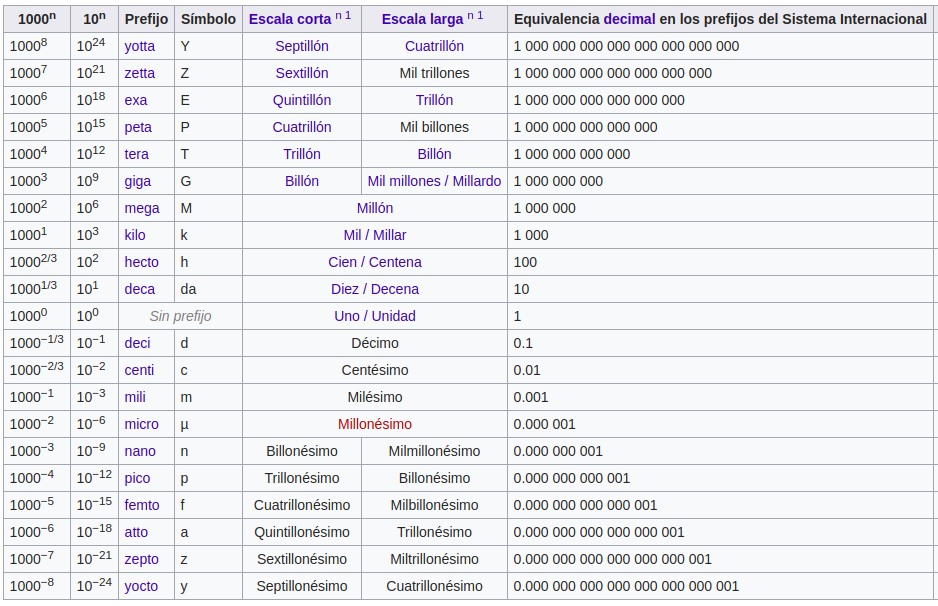
\includegraphics[scale=0.5]{img/prefijos.png}

\subsubsection{Notación científica}

\begin{myblock}{\textbf{Actividad \arabic{numact}}}
	Convierte las cantidades de notación científica a notación decimal o viceversa. 
	\textbf{Ejemplo}
	\begin{itemize}
		\item $0.0000067 \;[m] = 6.7 \times 10^{-6} \;[m] $
		\item $97 \times 10^{-3} \;[m] = 0.097 \;[m]$
	\end{itemize}

	
    
    \begin{multicols}{2} 
        \begin{enumerate}
            \item $986000 \;[m] $
            \item $0.000068 \;[m] $
            \item $0.0084 \;[m] $
            \item $0.34 \;[m] $
            \item $0.76 \times 10^{-7} \;[m] $
            \item $0.0078 \times 10^{-3} \;[m] $
            \item $0.00000007 \;[m] $
            \item $0.67 \times 10^{0}\;[m] $
            \item $12345 \times 10^{-1} \;[m] $
            \item $6731 \times 10^{-3}\;[m] $
            \item $4085 \times 10^{6} \;[m] $
            \item $15.14 \times 10^{3}\;[m] $
        \end{enumerate}
    \end{multicols}
\end{myblock}


\subsection{Clasificación de unidades}

\subsubsection{Unidades fundamentales y derivadas}

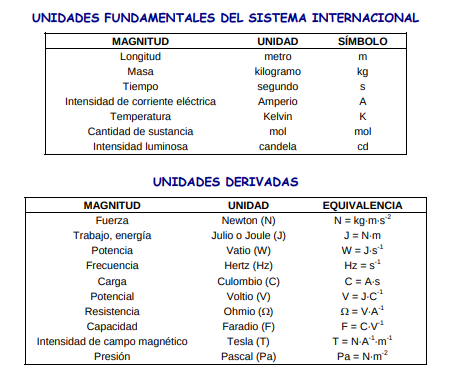
\includegraphics[scale=0.8]{img/unidades-fun_deriv.png}

\subsubsection{Unidades generales y especificas}

\subsection{Sistema de unidades}

\subsubsection{Sistema internacional de medidas}

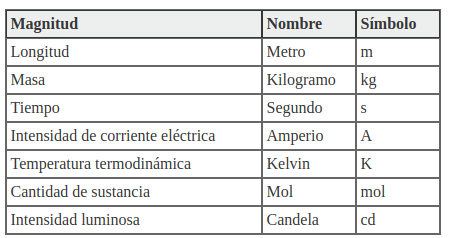
\includegraphics[scale=0.8]{img/si.png}

\subsubsection{Sistema cegesimal (cgs)}

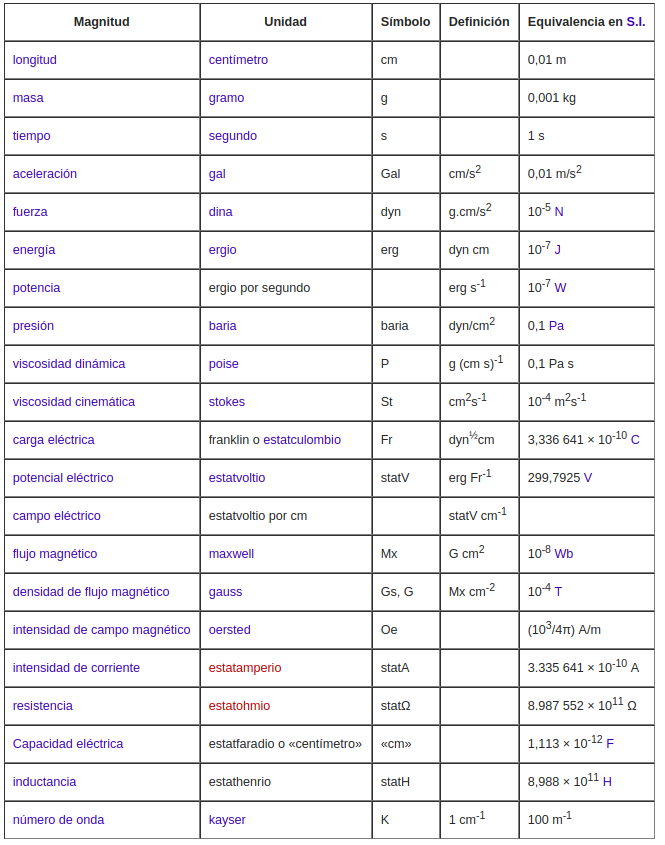
\includegraphics[scale=0.7]{img/cgs.png}

\subsubsection{Sistema inglés o imperial}

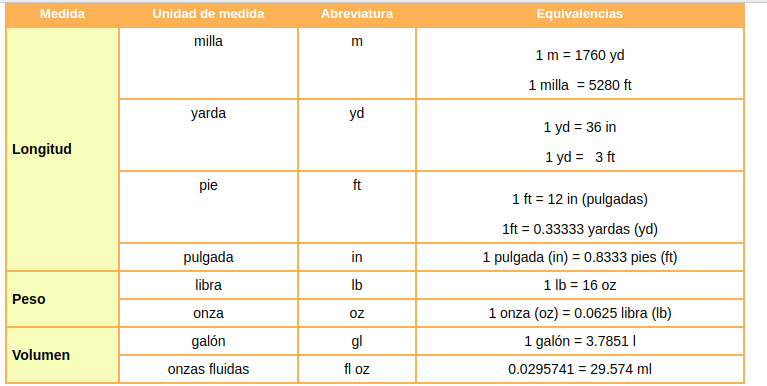
\includegraphics[scale=0.6]{img/singles.png}

%\subsubsection{Conversión de unidades}

\end{document}